\documentclass{beamer}
\usepackage{amsmath}
\usepackage{amsfonts}
\usepackage{amssymb}
\usepackage{natbib}
%\usepackage{fancyhdr}
%\usepackage[margin=1in]{geometry}
%%\usepackage{graphicx}
%%\usepackage{cite}
%%\usepackage{multicol}
%%\usepackage[section]{placeins}
%%\usepackage{amsthm}
\usepackage{nicefrac}
\usepackage{bm}
%%\usepackage{algorithm2e}
%\newtheorem{theorem}{Theorem}
%\newtheorem*{theorem*}{Theorem}
%\newtheorem{lemma}{Lemma}
%\newtheorem*{lemma*}{Lemma}
%\newtheorem*{def*}{Definition}
%\newtheorem*{conj}{Conjecture}
%\newtheorem{defn}{Definition}
%\newcommand{\low}[1]{$_{\text{#1}}$}
%\newcommand\xput[2][0.5]{%
%    \rule{#1\linewidth}{0pt}\makebox[0pt][c]{#2}\hfill}
%\usepackage{stackengine}
%\usepackage{enumerate}
\usepackage{tikz}
\usetikzlibrary{arrows.meta}
\usepackage{graphicx}
\usepackage{caption}
\usepackage{subcaption}

%
%\newcommand{\delt}[1]{
%\begin{tikzpicture}[#1]
%\draw (0,0) -- (1ex,1.5ex);
%\draw (2.1ex,0) -- (1ex,1.5ex);
%\draw (0.0,0.0) -- (2.1ex,0);
%\draw (0.5ex,0.8ex) -- (1.5ex, 0.8ex);
%\draw (1ex, 0.75ex) -- (1ex, 0);
%\end{tikzpicture}
%}
\usepackage[all]{xy}

\newcommand{\fp}{\varrho}
\newcommand{\nhalf}{\nicefrac{1}{2}}
%\newcommand{\eps}{\epsilon_{machine}}
\newcommand{\ol}{\overline}
\renewcommand{\b}{\bm}
%\newcommand{\problem}[2]{ \ \\\textbf{#1} \textit{#2}\\} 
%
\newcommand{\bE}{\mathbb{E}}
\newcommand{\bP}{\mathbb{P}}
\newcommand{\bR}{\mathbb{R}}
\newcommand{\bN}{\mathbb{N}}
\newcommand{\bZ}{\mathbb{Z}}
\newcommand{\bQ}{\mathbb{Q}}
\newcommand{\bC}{\mathbb{C}}
\newcommand{\cA}{\mathcal{A}}
\newcommand{\cB}{\mathcal{B}}
\newcommand{\cC}{\mathcal{C}}
\newcommand{\cD}{\mathcal{D}}
\newcommand{\cE}{\mathcal{E}}
\newcommand{\cF}{\mathcal{F}}
\newcommand{\cG}{\mathcal{G}}
\newcommand{\cH}{\mathcal{H}}
\newcommand{\cI}{\mathcal{I}}
\newcommand{\cJ}{\mathcal{J}}
\newcommand{\cK}{\mathcal{K}}
\newcommand{\cL}{\mathcal{L}}
\newcommand{\cM}{\mathcal{M}}
\newcommand{\cN}{\mathcal{N}}
\newcommand{\cO}{\mathcal{O}}
\newcommand{\cP}{\mathcal{P}}
\newcommand{\cQ}{\mathcal{Q}}
\newcommand{\cR}{\mathcal{R}}
\newcommand{\cS}{\mathcal{S}}
\newcommand{\cT}{\mathcal{T}}
\newcommand{\cU}{\mathcal{U}}
\newcommand{\cV}{\mathcal{V}}
\newcommand{\cW}{\mathcal{W}}
\newcommand{\cX}{\mathcal{X}}
\newcommand{\cY}{\mathcal{Y}}
\newcommand{\cZ}{\mathcal{Z}}

\definecolor{lblue}{RGB}{51,255,255}
\definecolor{dgreen}{RGB}{49,128,23}
\definecolor{nicepink}{RGB}{255, 0, 102}
\definecolor{nicered}{RGB}{255, 100, 100}
\definecolor{niceredL}{RGB}{255, 150,150}
\definecolor{niceredH}{RGB}{255, 20, 20}
\definecolor{lblue}{RGB}{102, 163, 255}
\definecolor{lgray}{RGB}{217, 217, 217}


\newcommand{\kr}{\text{k}}
%
%\renewcommand{\arraystretch}{1.5}
%\renewcommand{\thefootnote}{\fnsymbol{footnote}}	
%\setlength{\headheight}{5pt}
%\pagestyle{fancyplain}
%\renewcommand{\headrulewidth}{0pt}
%\lhead{}
%\chead{}
%\rhead{}

%\lfoot{}
%\cfoot{\thepage}
%\rfoot{}

\setbeamerfont{block body}{size=\small}

\usetheme{Ilmenau}
\usecolortheme{seahorse}
\usefonttheme{serif}

\addtobeamertemplate{navigation symbols}{}{%
    \usebeamerfont{footline}%
    \usebeamercolor[fg]{footline}%
    \hspace{1em}%
    \insertframenumber/\inserttotalframenumber
}

\author[Brunner]{Jim Brunner}
\institute[LANL]{Los Alamos National Laboratory}
\title{Using Cooccurrance Networks}
\date{}
\begin{document}
%--------------------------------------------------------------------------------------------------
\begin{frame}
\titlepage
%\phantom{\cite{}}
\end{frame}
%--------------------------------------------------------------------------------------------------
\begin{frame}
\frametitle{Coincidence Network}
Constructing a coincidence network.
I map the abundances according to
\[
a(r_{ji})  = \left\{
\begin{array}{c c}
\lfloor\left(\frac{r_{ji}}{\max_{s_k}(r_{jk})}\right) n \rfloor + 1 &  \frac{r_{ji}}{\max_{s_k}(r_{jk})} \geq m \\
0 & \frac{r_{ji}}{\max_{s_k}(r_{jk})} < m
\end{array}
\right.
\]
into ``bins" relative to the maximum that taxa appears. Then count 
\[
w^1_{jk} = \frac{\|\{i: a(r_{ji}) = a(r_{ki}) \neq 0\} \|}{S}
\]
how often two organisms appear in the same bin.
\end{frame}
%--------------------------------------------------------------------------------------------------
%--------------------------------------------------------------------------------------------------
\begin{frame}
\frametitle{Cooccurrance Network}
Same idea but now edges weights are compared to a random graph (null model). 
So we only keep edges that have a higher than ``random" weight.
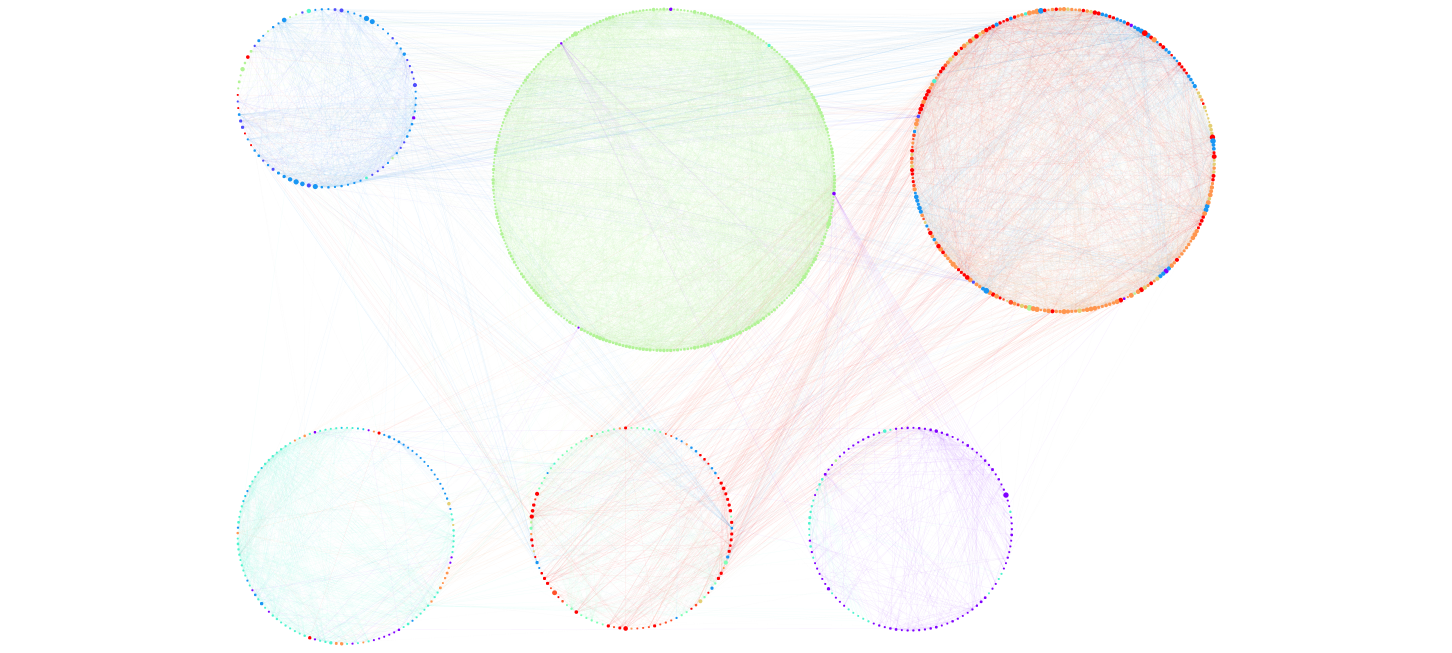
\includegraphics[scale = 0.2]{../../../old_networks/june20/june20_species.png}
\end{frame}
%--------------------------------------------------------------------------------------------------
%--------------------------------------------------------------------------------------------------
\begin{frame}
\frametitle{Cooccurrance Network - Pearson Correlation}
We can also compute the Pearson correlation coefficient between taxa across the samples. 
\[
\rho_{xy} = \frac{1}{N}\frac{(\b{x}- \mu_x\b{1}) \cdot (\b{y} - \mu_y\b{1})}{\sigma_x \sigma_y}
\]
Then, we keep an edge if $\rho > 0.8$ and $p< 0.05$, where $p$ is the chance of correlation higher than $\rho_{xy}$ in a random model. The random model assigns abundances as a binomial with parameters determined by sample and taxa. The $p$ values are calculated using a Monte Carlo simulation with 1000 trials. 

The species level network using this method had $\sim \nhalf$ as many edges.
\end{frame}
%--------------------------------------------------------------------------------------------------
%--------------------------------------------------------------------------------------------------
\begin{frame}
\frametitle{Cooccurrance Network - Pearson Correlation}
\begin{center}
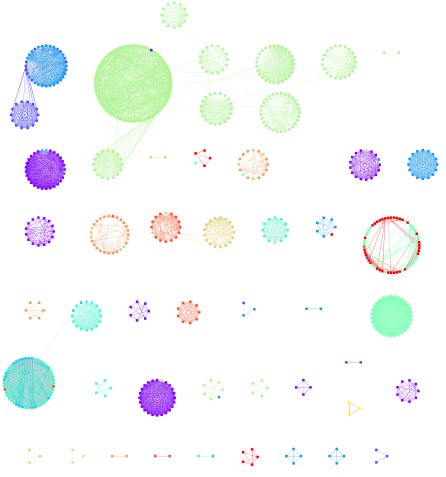
\includegraphics[scale = 0.4]{../pearson_species.png}
\end{center}
\end{frame}
%--------------------------------------------------------------------------------------------------
%--------------------------------------------------------------------------------------------------
\begin{frame}
\frametitle{Clustering}
We can cluster the network to attempt to determine or evaluate meaningful groups of taxa.
\begin{itemize}
	\item Community clustering
	\begin{itemize}\item Minimize a function based on ``edge betweeness". Determines edges that are between clusters.\end{itemize}
	\item Spectral clustering
	\begin{itemize}
		\item Performs a random walk on the network.
	\end{itemize} 
\end{itemize}
\end{frame}
%--------------------------------------------------------------------------------------------------
%--------------------------------------------------------------------------------------------------
\begin{frame}
\frametitle{Analyzing a sample}
\begin{itemize}
	\item Filter GOTTCHA results - try to determine probability of seeing groups of organisms - Random Markov Field
 	\item Diffusion on graph
\end{itemize}
\[
\frac{\partial}{\partial t} u(v,t) = -L u(v,t)
\]
where $v$ takes values in the vertex set of the graph. Then, we can encode ``known" information in three ways: initial values, boundary values, or a forcing vector.



\end{frame}
%--------------------------------------------------------------------------------------------------
%--------------------------------------------------------------------------------------------------
\begin{frame}
\frametitle{Analyzing a sample - Diffusion Process}
\[
\frac{\partial}{\partial t} u(v,t) = -L u(v,t)
\]
where $v$ takes values in the vertex set of the graph. Then, we can encode sample information in three ways: initial values, boundary values, or a forcing vector.

\medskip
Related to spectral clustering - spectral clustering groups by ``distance" in firsk $k$ eigenmodes of diffusion process. This process gives ``distance" in weighted sum of eigenmodes of diffusion process.

\medskip
{\bf Highest ranked nodes are ``closest" to the sample data}



\end{frame}
%--------------------------------------------------------------------------------------------------
%--------------------------------------------------------------------------------------------------
\begin{frame}
\frametitle{Initial Values}
\begin{block}{Initial Value Problem}
	Let $u_i(t)$ be the solution at node $v_i$ to the discete diffusion problem
	\[
	\frac{d}{dt}\b{u}(t)  = - L\b{u}
	\]
	where $L$ is the  graph laplacian with initial conditions determined by sample information.
	
	Then, if $\b{K}$ is the information ``known" from the sample and the values of $v_{k}$ and $v_{l}$ are unknown,
	\[
	\int_0^{\infty} u_k(t) dt - \int_0^{\infty} u_l(t) dt >  0 \Rightarrow  P(v_k=  1|\b{K}) > P(v_l = 1|\b{K})
	\]
\end{block}
\end{frame}
%--------------------------------------------------------------------------------------------------
%--------------------------------------------------------------------------------------------------
\begin{frame}
\frametitle{Boundary Values}
	\begin{block}{Boundary Value Problem}
	Let $u_i(t)$ be the solution at node $v_i$ to the discete diffusion problem
	\[
	\frac{d}{dt}\b{u}(t)  = - L\b{u}
	\]
	where $L$ is the  graph laplacian with fixed values (which can be regarded as boundary values) $u_i = 1$ if node $v_i$ is known to be ``on", $u_j = 0$ if $v_j$ is known to be ``off". 
	
	Then, if $\b{K}$ is the information ``known" and the values of $v_{k}$ and $v_{l}$ are unknown, and $\b{\tilde{u}}$ is the equilibrium solution to the diffusion problem,
	\[
	\tilde{u}_k dt >  \tilde{u}_l \Leftrightarrow  P(v_k=  1|\b{K}) > P(v_l = 1|\b{K})
	\]
\end{block}
\end{frame}
%--------------------------------------------------------------------------------------------------
%--------------------------------------------------------------------------------------------------
\begin{frame}
\frametitle{Forcing Function}
\begin{block}{Forced Problem}
	Let $u_i(t)$ be the solution at node $v_i$ to the discete diffusion problem
	\[
	\frac{d}{dt}\b{u}(t)  = - L\b{u} + f
	\]
	where $L$ is the  graph laplacian and $f$ a forcing vector with $f_i = \alpha_{cc}$ if node $v_i$ is known to be ``on", $f_j = -\beta_{cc}$ if $v_j$ is known to be ``off", where $cc$ denotes a connected component of the graph. We choose $\alpha_{cc}$ and $\beta_{cc}$ so that on any connected component $cc$, $\sum \alpha_{cc}= \sum \beta_{cc}= 1$. 
	
	Then, if $\b{K}$ is the information ``known" and the values of $v_{k}$ and $v_{l}$ are unknown, and $\b{\tilde{u}}$ is the equilibrium solution to the diffusion problem,
	\[
	\tilde{u}_k dt >  \tilde{u}_l \Leftrightarrow  P(v_k=  1|\b{K}) > P(v_l = 1|\b{K})
	\]
\end{block}
\end{frame}
%--------------------------------------------------------------------------------------------------
%--------------------------------------------------------------------------------------------------
\begin{frame}
\frametitle{Small Network Examples}
\begin{figure}
	\begin{subfigure}[b]{0.3\linewidth}
		\begin{center}
			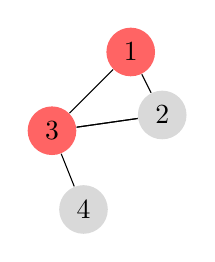
\begin{tikzpicture}[scale = 1]
			\node (a) at (1,2) [circle, fill = nicered] {$1$};
			\node (b) at (1.4,1.2) [circle, fill = lgray] {$2$};
			\node (c) at (0,1) [circle, fill = nicered] {$3$};
			\node (d) at (0.4,0) [circle, fill = lgray] {$4$};
			\draw (b) edge (c);
			\draw (a) edge (b);
			\draw (a) edge (c);
			\draw (b) edge (c);
			\draw (c) edge (d);
			\end{tikzpicture}
		\end{center}
		\caption{Small network, two on.}
	\end{subfigure}
	\begin{subfigure}[b]{0.3\linewidth}
		\begin{center}
			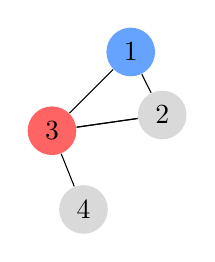
\begin{tikzpicture}[scale = 1]
			\node (a) at (1,2) [circle, fill = lblue] {$1$};
			\node (b) at (1.4,1.2) [circle, fill = lgray] {$2$};
			\node (c) at (0,1) [circle, fill = nicered] {$3$};
			\node (d) at (0.4,0) [circle, fill = lgray] {$4$};
			\draw (b) edge (c);
			\draw (a) edge (b);
			\draw (a) edge (c);
			\draw (b) edge (c);
			\draw (c) edge (d);
			\end{tikzpicture}
		\end{center}
		\caption{small network, one on one off}
	\end{subfigure}
	\begin{subfigure}[b]{0.3\linewidth}
		\begin{center}
			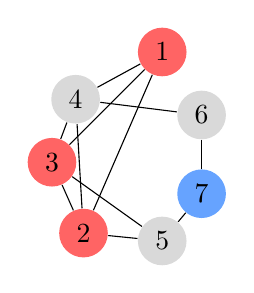
\begin{tikzpicture}[scale = 1]
			\node (a) at (1,2.3) [circle, fill = nicered] {$1$};
			\node (b) at (0,0) [circle, fill = nicered] {$2$};
			\node (c) at (-0.4,0.9) [circle, fill = nicered] {$3$};
			\node (d) at (-0.1,1.7) [circle, fill = lgray] {$4$};
			\node (e) at (1,-0.1) [circle, fill = lgray] {$5$};
			\node (f) at (1.5,1.5) [circle, fill = lgray] {$6$};
			\node (g) at (1.5,0.5)[circle, fill = lblue] {$7$};
			\draw (a) edge (b);
			\draw (a) edge (c);
			\draw (a) edge (d);
			\draw (b) edge (c);
			\draw (b) edge (d);
			\draw (c) edge (d);
			\draw (d) edge (f);
			\draw (f) edge (g);
			\draw (e) edge (g);
			\draw (c) edge (e);
			\draw (b) edge (e);
			\end{tikzpicture}
		\end{center}
		\caption{Larger network}
	\end{subfigure}
	\caption{Test networks. Gray nodes were ``unknown", blue nodes ``off", and red ``on".}
\end{figure}
\end{frame}
%--------------------------------------------------------------------------------------------------
%--------------------------------------------------------------------------------------------------
\begin{frame}
\frametitle{Small Network Examples}
	\begin{center}
		\begin{tabular}{|l|l|l|l|}
			\hline Configuration & Method & Ranking & Ties\\
			\hline
			(a) Small Network, two on. &  IVP & 2, 4 & none  \\ \cline{2-4}
			& BVP & 4, 2 & 4, 2 \\ \cline{2-4}
			& Forcing & 2, 4 & none \\
			\hline
			(b) Small Network, one on one off &  IVP & 4, 2 &none \\ \cline{2-4}
			& BVP &4, 2 & none  \\ \cline{2-4}
			& Forcing &4, 2 & none\\
			\hline
			(c) Larger network &  IVP & 4, 5, 6& none \\ \cline{2-4}
			& BVP & 4, 5, 6&  none\\ \cline{2-4}
			& Forcing &  4, 5, 6& none \\
			\hline
		\end{tabular}
	\end{center}
\end{frame}
%--------------------------------------------------------------------------------------------------
%--------------------------------------------------------------------------------------------------
\begin{frame}
\frametitle{Network Examples}
\begin{figure}
		\begin{center}
	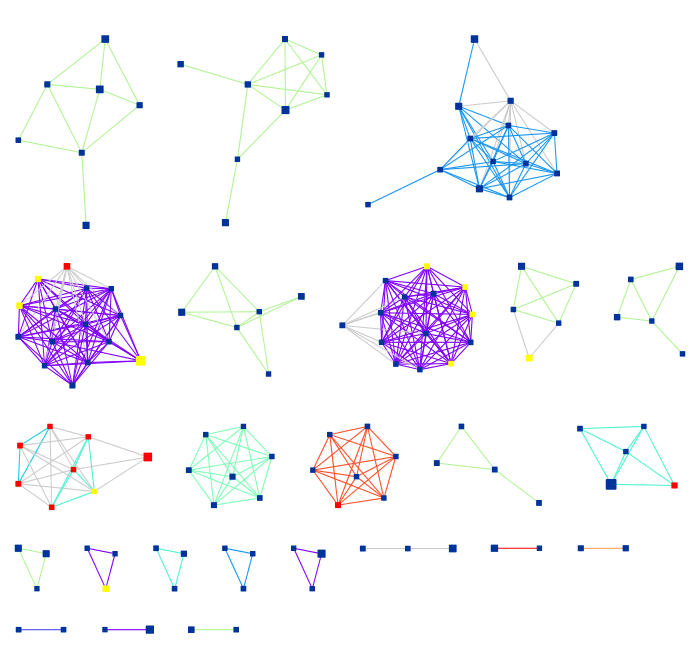
\includegraphics[scale = 0.25]{../ranked_known_nodes.png}	
\end{center}
\caption{The ``known" set - blue is off and red is on, while yellow is unknown.}
\end{figure}
\end{frame}
%--------------------------------------------------------------------------------------------------
%--------------------------------------------------------------------------------------------------
\begin{frame}
\frametitle{Network Examples}
	\begin{figure}
	\begin{center}
		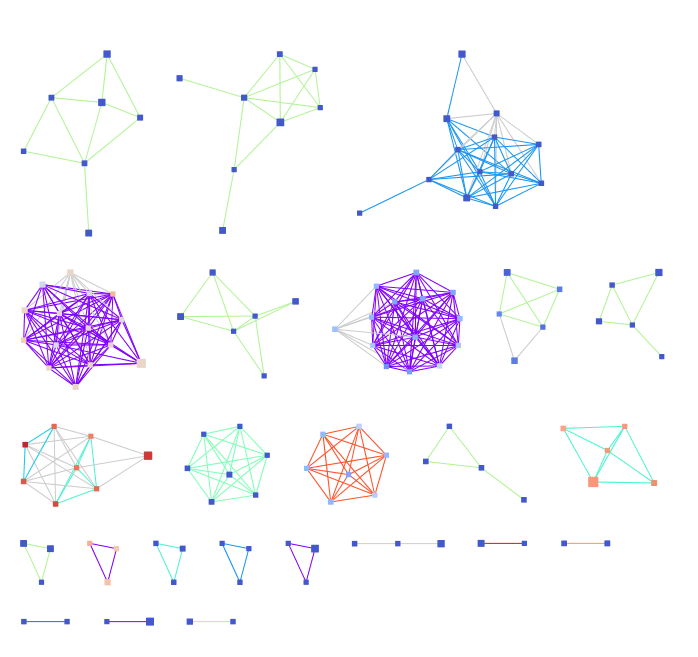
\includegraphics[scale = 0.25]{../ranked_ivp.png}	
	\end{center}
	\caption{Result of initial value problem, with all nodes analyzed. Hotter colors indicate higher likelihood.}
\end{figure}
\end{frame}
%--------------------------------------------------------------------------------------------------
%--------------------------------------------------------------------------------------------------
\begin{frame}
\frametitle{Network Examples}
\begin{figure}
	\begin{center}
	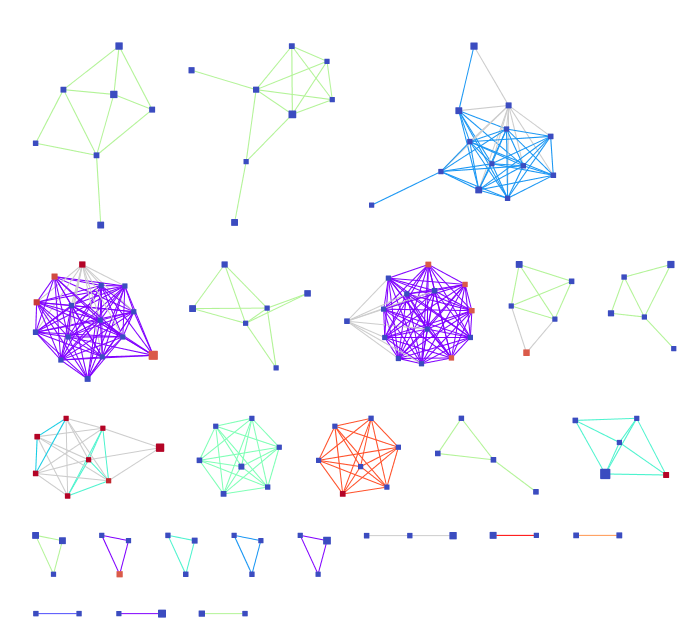
\includegraphics[scale = 0.25]{../ranked_bdvp.png}	
\end{center}
\caption{Result of boundary value problem. Hotter colors indicate higher likelihood, with red indicating assumed ``on".}
\end{figure}
\end{frame}
%--------------------------------------------------------------------------------------------------
%--------------------------------------------------------------------------------------------------
\begin{frame}
\frametitle{Assigning a sample}
 Given a sample, we get ranking from a network $N_j$. Let $\b{r}^j(\b{s})$ be the ranking given by diffusion on network $j$. Then,
\[
F_j(\b{s}) = F(\b{s},\b{r}^j(\b{s})) = \sum_{i=1}^n c^{r_i^j} \frac{s_i}{\|\b{s}\|_1}
\]
and we can attempt to optimize over the networks we have (if there's only a few that's easy). The conjecture is then
\begin{block}{Conjecture}
	Assume that $F_j(\b{s}) > F_k(\b{s})$. Then $P(\b{s}|N_j) > P(\b{s}|N_k)$.
\end{block}
\end{frame}
%--------------------------------------------------------------------------------------------------
%--------------------------------------------------------------------------------------------------
\begin{frame}
\frametitle{Assigning a sample}
\begin{figure}
	\begin{subfigure}[b]{0.46\linewidth}
		\begin{center}
			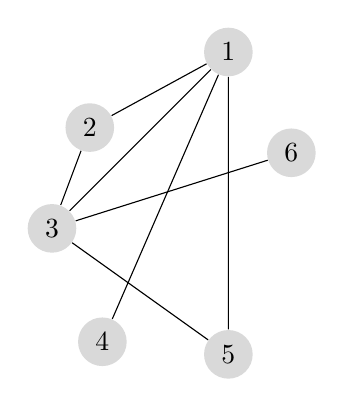
\begin{tikzpicture}[scale = 1.6]
			\node (a) at (1,2.3) [circle, fill = lgray] {$1$};
			\node (d) at (0,0) [circle, fill = lgray] {$4$};
			\node (c) at (-0.4,0.9) [circle, fill = lgray] {$3$};
			\node (b) at (-0.1,1.7) [circle, fill = lgray] {$2$};
			\node (e) at (1,-0.1) [circle, fill = lgray] {$5$};
			\node (f) at (1.5,1.5) [circle, fill = lgray] {$6$};
			\draw (a) edge (b);
			\draw (a) edge (c);
			\draw (b) edge (c);
			\draw (a) edge (d);
			\draw (a) edge (e);
			\draw (c) edge (f);
			\draw (c) edge (e);
			\end{tikzpicture}
		\end{center}
		\caption{Network $A_1$}
	\end{subfigure}
	\begin{subfigure}[b]{0.46\linewidth}
		\begin{center}
			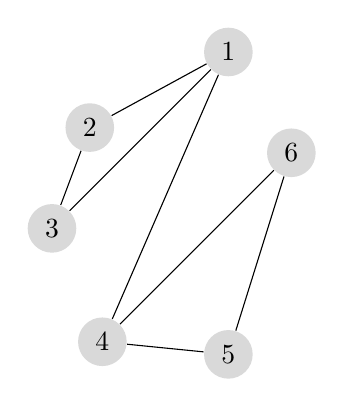
\begin{tikzpicture}[scale = 1.6]
			\node (a) at (1,2.3) [circle, fill = lgray] {$1$};
			\node (d) at (0,0) [circle, fill = lgray] {$4$};
			\node (c) at (-0.4,0.9) [circle, fill = lgray] {$3$};
			\node (b) at (-0.1,1.7) [circle, fill = lgray] {$2$};
			\node (e) at (1,-0.1) [circle, fill = lgray] {$5$};
			\node (f) at (1.5,1.5) [circle, fill = lgray] {$6$};
			\draw (a) edge (b);
			\draw (a) edge (c);
			\draw (b) edge (c);
			\draw (a) edge (d);
			\draw (e) edge (d);
			\draw (d) edge (f);
			\draw (f) edge (e);
			\end{tikzpicture}
		\end{center}
		\caption{Network $A_2$}
	\end{subfigure}
	\caption{Test Networks}
\end{figure}
\end{frame}
%--------------------------------------------------------------------------------------------------
%--------------------------------------------------------------------------------------------------
\begin{frame}
\frametitle{Assigning a sample}
\begin{figure}
	\begin{subfigure}[b]{0.46\linewidth}
		\begin{center}
			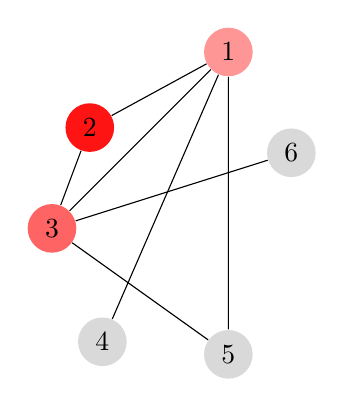
\begin{tikzpicture}[scale = 1.6]
			\node (a) at (1,2.3) [circle, fill = niceredL] {$1$};
			\node (d) at (0,0) [circle, fill = lgray] {$4$};
			\node (c) at (-0.4,0.9) [circle, fill = nicered] {$3$};
			\node (b) at (-0.1,1.7) [circle, fill = niceredH] {$2$};
			\node (e) at (1,-0.1) [circle, fill = lgray] {$5$};
			\node (f) at (1.5,1.5) [circle, fill = lgray] {$6$};
			\draw (a) edge (b);
			\draw (a) edge (c);
			\draw (b) edge (c);
			\draw (a) edge (d);
			\draw (a) edge (e);
			\draw (c) edge (f);
			\draw (c) edge (e);
			\end{tikzpicture}
		\end{center}
		\caption{Network $A_1$}
	\end{subfigure}
	\begin{subfigure}[b]{0.46\linewidth}
		\begin{center}
			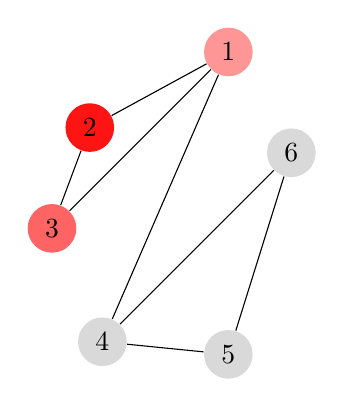
\begin{tikzpicture}[scale = 1.6]
			\node (a) at (1,2.3) [circle, fill = niceredL] {$1$};
			\node (d) at (0,0) [circle, fill = lgray] {$4$};
			\node (c) at (-0.4,0.9) [circle, fill = nicered] {$3$};
			\node (b) at (-0.1,1.7) [circle, fill = niceredH] {$2$};
			\node (e) at (1,-0.1) [circle, fill = lgray] {$5$};
			\node (f) at (1.5,1.5) [circle, fill = lgray] {$6$};
			\draw (a) edge (b);
			\draw (a) edge (c);
			\draw (b) edge (c);
			\draw (a) edge (d);
			\draw (e) edge (d);
			\draw (d) edge (f);
			\draw (f) edge (e);
			\end{tikzpicture}
		\end{center}
		\caption{Network $A_2$}
	\end{subfigure}
	\caption{``Sample" $u_1 = (\nicefrac{1}{6},\nhalf,\nicefrac{1}{3},0,0,0)$}
\end{figure}
\end{frame}
%--------------------------------------------------------------------------------------------------
%--------------------------------------------------------------------------------------------------
\begin{frame}
\frametitle{Assigning a sample}
\begin{figure}
	\begin{subfigure}[b]{0.46\linewidth}
		\begin{center}
			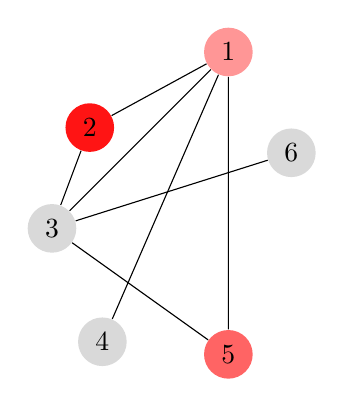
\begin{tikzpicture}[scale = 1.6]
			\node (a) at (1,2.3) [circle, fill = niceredL] {$1$};
			\node (d) at (0,0) [circle, fill = lgray] {$4$};
			\node (c) at (-0.4,0.9) [circle, fill = lgray] {$3$};
			\node (b) at (-0.1,1.7) [circle, fill = niceredH] {$2$};
			\node (e) at (1,-0.1) [circle, fill = nicered] {$5$};
			\node (f) at (1.5,1.5) [circle, fill = lgray] {$6$};
			\draw (a) edge (b);
			\draw (a) edge (c);
			\draw (b) edge (c);
			\draw (a) edge (d);
			\draw (a) edge (e);
			\draw (c) edge (f);
			\draw (c) edge (e);
			\end{tikzpicture}
		\end{center}
		\caption{Network $A_1$}
	\end{subfigure}
	\begin{subfigure}[b]{0.46\linewidth}
		\begin{center}
			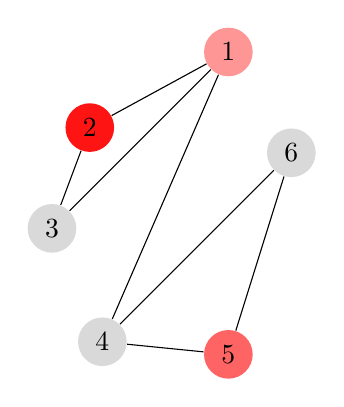
\begin{tikzpicture}[scale = 1.6]
			\node (a) at (1,2.3) [circle, fill = niceredL] {$1$};
			\node (d) at (0,0) [circle, fill = lgray] {$4$};
			\node (c) at (-0.4,0.9) [circle, fill = lgray] {$3$};
			\node (b) at (-0.1,1.7) [circle, fill = niceredH] {$2$};
			\node (e) at (1,-0.1) [circle, fill = nicered] {$5$};
			\node (f) at (1.5,1.5) [circle, fill = lgray] {$6$};
			\draw (a) edge (b);
			\draw (a) edge (c);
			\draw (b) edge (c);
			\draw (a) edge (d);
			\draw (e) edge (d);
			\draw (d) edge (f);
			\draw (f) edge (e);
			\end{tikzpicture}
		\end{center}
		\caption{Network $A_2$}
	\end{subfigure}
	\caption{``Sample" $u_2 = (\nicefrac{1}{6},\nhalf,0,0,\nicefrac{1}{3},0)$}
\end{figure}
\end{frame}
%--------------------------------------------------------------------------------------------------
%--------------------------------------------------------------------------------------------------
\begin{frame}
\frametitle{Assigning a sample}
\begin{figure}
	\begin{subfigure}[b]{0.46\linewidth}
		\begin{center}
			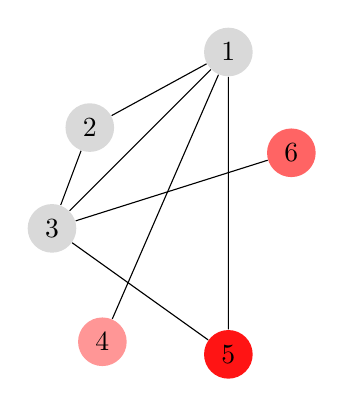
\begin{tikzpicture}[scale = 1.6]
			\node (a) at (1,2.3) [circle, fill = lgray] {$1$};
			\node (d) at (0,0) [circle, fill = niceredL] {$4$};
			\node (c) at (-0.4,0.9) [circle, fill = lgray] {$3$};
			\node (b) at (-0.1,1.7) [circle, fill = lgray] {$2$};
			\node (e) at (1,-0.1) [circle, fill = niceredH] {$5$};
			\node (f) at (1.5,1.5) [circle, fill = nicered] {$6$};
			\draw (a) edge (b);
			\draw (a) edge (c);
			\draw (b) edge (c);
			\draw (a) edge (d);
			\draw (a) edge (e);
			\draw (c) edge (f);
			\draw (c) edge (e);
			\end{tikzpicture}
		\end{center}
		\caption{Network $A_1$}
	\end{subfigure}
	\begin{subfigure}[b]{0.46\linewidth}
		\begin{center}
			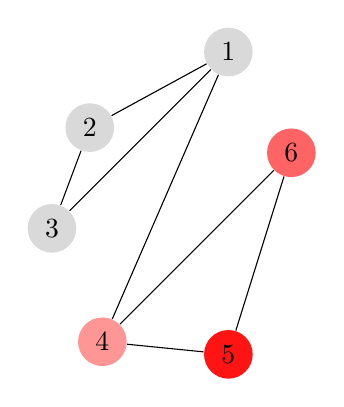
\begin{tikzpicture}[scale = 1.6]
			\node (a) at (1,2.3) [circle, fill = lgray] {$1$};
			\node (d) at (0,0) [circle, fill = niceredL] {$4$};
			\node (c) at (-0.4,0.9) [circle, fill = lgray] {$3$};
			\node (b) at (-0.1,1.7) [circle, fill = lgray] {$2$};
			\node (e) at (1,-0.1) [circle, fill = niceredH] {$5$};
			\node (f) at (1.5,1.5) [circle, fill = nicered] {$6$};
			\draw (a) edge (b);
			\draw (a) edge (c);
			\draw (b) edge (c);
			\draw (a) edge (d);
			\draw (e) edge (d);
			\draw (d) edge (f);
			\draw (f) edge (e);
			\end{tikzpicture}
		\end{center}
		\caption{Network $A_2$}
	\end{subfigure}
	\caption{``Sample" $u_3= (0,0,0,\nicefrac{1}{6},\nhalf,\nicefrac{1}{3})$}
\end{figure}
\end{frame}
%--------------------------------------------------------------------------------------------------
%--------------------------------------------------------------------------------------------------
\begin{frame}
\frametitle{Assigning a sample}

	\begin{center}
		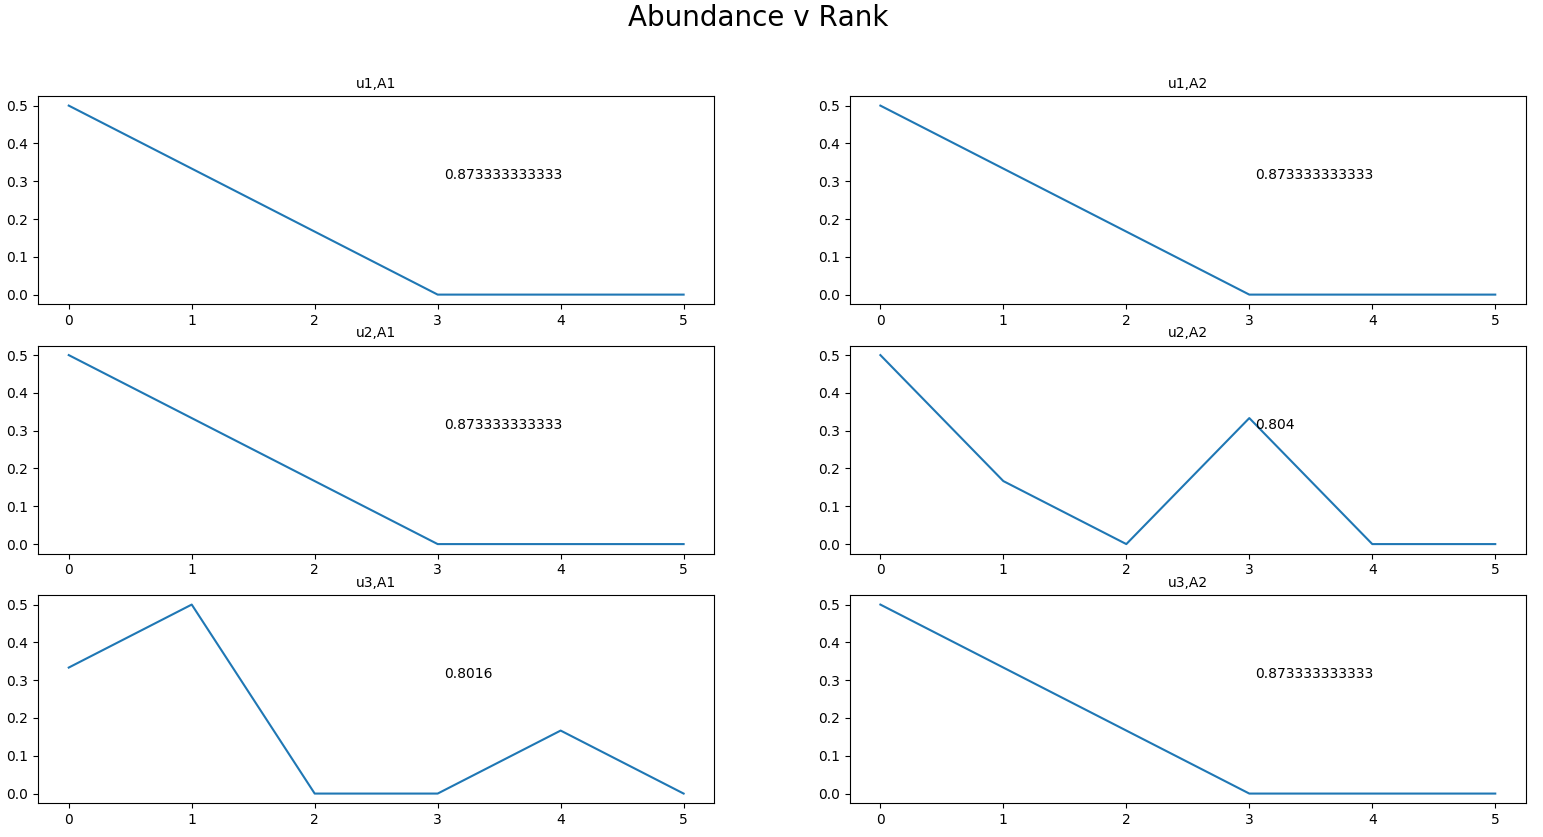
\includegraphics[scale = 0.3]{../tiny.png}	
	\end{center}

\end{frame}
%--------------------------------------------------------------------------------------------------
%--------------------------------------------------------------------------------------------------
\begin{frame}
\frametitle{Assigning a sample}

	\begin{center}
		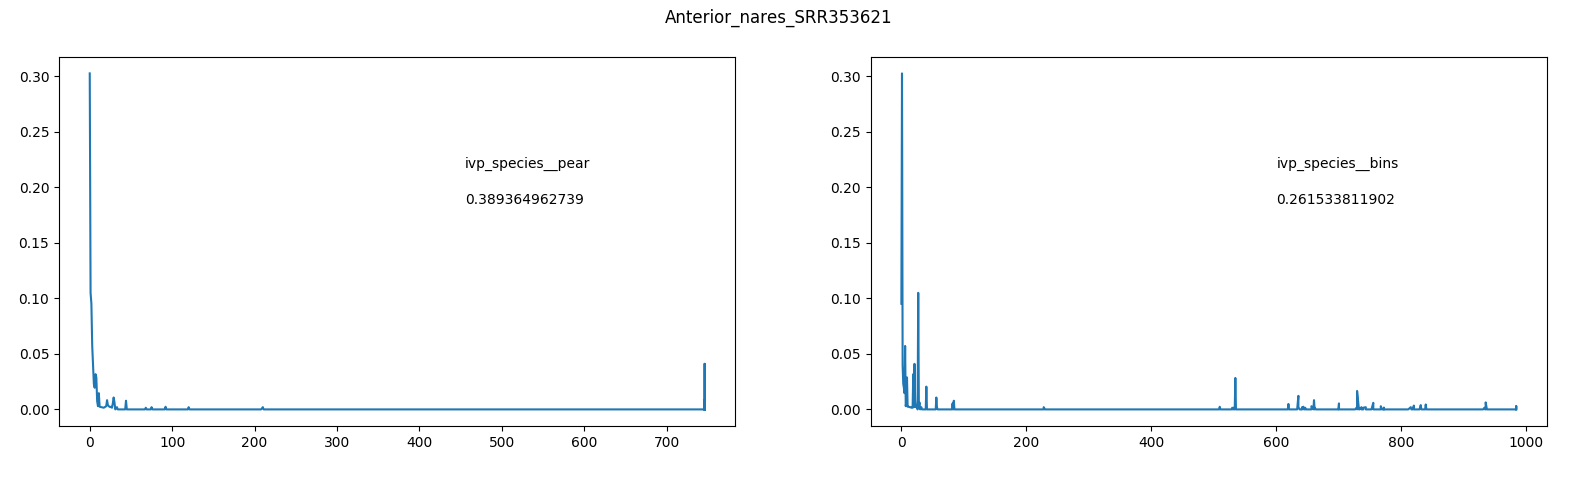
\includegraphics[scale = 0.25]{../a_nares.png}	
	\end{center}

	\begin{center}
	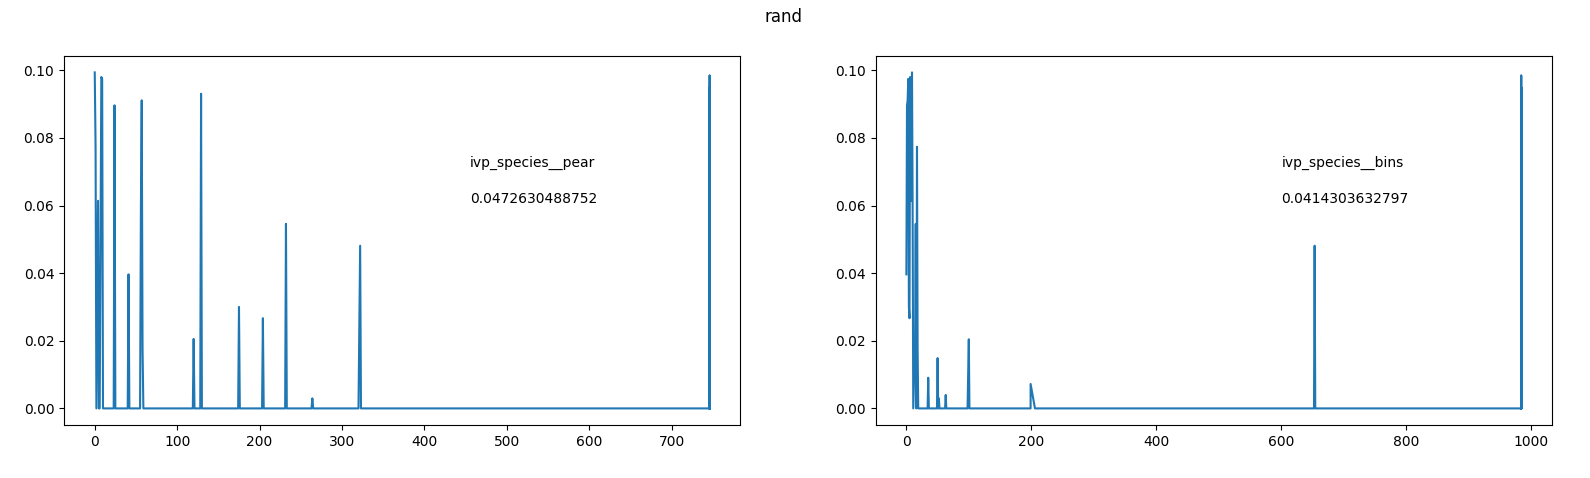
\includegraphics[scale = 0.25]{../random.png}	
\end{center}

\end{frame}
%--------------------------------------------------------------------------------------------------
%--------------------------------------------------------------------------------------------------

%\begin{frame}
%\frametitle{References}
%\bibliographystyle{unsrt}
%% make bibliography entries smaller
%\renewcommand\bibfont{\scriptsize}
%% and kill the abominable icon
%\setbeamertemplate{bibliography item}{}
%\bibliography{../summer17}
%\end{frame}
%%--------------------------------------------------------------------------------------------------
%--------------------------------------------------------------------------------------------------
%\begin{frame}
%\frametitle{Thank You}
%
%
%\end{frame}
%%--------------------------------------------------------------------------------------------------
\end{document}